\chapter{Teaching Your PI Controller to Behave (Part III)}\label{ch:3}

In my last blog, I explained how to calculate the P and I coefficients (actually the $K_a$ and $K_b$ coefficients in a series structure) for a current loop PI controller for a motor.  We saw that Kb could be used to eliminate the zero in the closed-loop system response, resulting in a system having only one real pole (i.e., well behaved and stable).  $K_a$ sets the bandwidth of the closed-loop system response.

Today, let’s back out and take a look at a speed control loop which contains two PI controllers; one to control the motor’s current, and another to control the motor’s speed.  From the figure below, notice that the output of the velocity PI controller is connected as the input reference signal for the PI current controller.  This makes sense when you think about it.  If the velocity is too low, we want to increase the motor’s current to produce more torque to speed it up.  Conversely if the motor is going too fast, we want to decrease the motor’s torque (or even drive it negative) to slow the motor down.  Together, these two PI controllers form a cascaded control loop.  By “cascaded,” I mean a control system that consists of an outer loop with one or more inner loops.  In my last blog, we saw that setting the coefficients for the PI current controller is a fairly deterministic process.  Can designing the speed PI controller be just as simple?  Do the coefficient values perform the same system functions they did with the current controller?

It turns out that closing the speed loop is a little more complicated than closing the current loop.  To properly design the speed loop, we need to know more system parameters than we did for the current loop.  This can be seen in the figure below which shows all of the components that comprise a typical cascaded speed control loop.


\begin{center}
    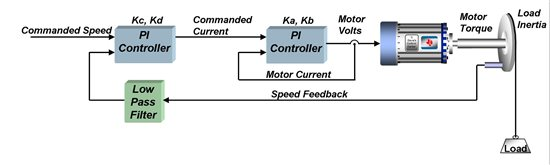
\includegraphics[width=1\linewidth]{03/01}
\end{center}

Notice that in our system, the speed feedback signal is filtered.  Unless you have an analog tachometer mounted to your motor shaft, you are probably synthesizing the speed signal by measuring other system parameters.  Even if you are using an incremental encoder on the motor shaft, you will need to synthesize velocity by measuring position.  For this reason, the speed signal often needs to be filtered before it is usable by the control system.  For our purposes, let’s just assume that we are using a single-pole low pass filter of the form:

\begin{equation}\label{eq:3_1}
    Vel_{filter}(s) = \frac{1}{\tau s+1}
\end{equation}

where $\tau$ is the time constant of the velocity filter.

Assuming we design the current loop as discussed in my previous blog, its closed-loop transfer function is:

\begin{equation}\label{eq:3_2}
    G_{current}(s) = \frac{1}{\frac{L}{K_a}s+1}
\end{equation}

where $K_a$ is the error gain term in the current regulator’s PI structure.  Recall that $K_b$ is not visible to the speed loop since it is used internally to the current loop to achieve pole-zero cancellation in its closed-loop transfer function.

I hate to do this to you again, but we are going to have to wade through a little bit more math to understand how to set the two coefficients for the speed PI controller.  To avoid confusing the coefficients of the speed controller with those of the current controller, we will call the speed controller’s coefficients $K_c$ and $K_d$ as shown in the figure above.  In the series form of the PI controller, $K_c$ will be the error gain term ($K_c = K_p$), and $K_d$ is the integrator gain term ($K_d = K_i/K_p$).  So let’s use the same equation I did in my last blog for the current controller to define the transfer function for the speed PI controller:

\begin{equation}\label{eq:3_3}
    PI_{speed}(s) = \frac{K_cK_d}{s}+K_c = \frac{K_cK_d\left(1+\frac{s}{K_d}\right)}{s}
\end{equation}

The transfer function from motor current to motor torque will vary as a function of what type of motor you are using.  Assuming we are using a Permanent Magnet Synchronous Motor under Field Oriented Control, the transfer function between q-axis current and motor torque is:

\begin{equation}\label{eq:3_4}
    Mtr(s) = \frac{3}{2}\frac{P}{2}\lambda_r = \frac{3}{4}P \lambda _r
\end{equation}
where $P = \text{the number of rotor poles}$ and $\lambda_r = \text{the rotor flux}$ (which is also equal to the back-EMF constant ($K_e$) in SI units)
\\

For reference sake, an AC Induction motor has a little bit different transfer function between q-axis current and motor torque:

\begin{equation*}
    Mtr(s) = \frac{3}{4}P \frac{}{L_m^2}{L_r}I_d
\end{equation*}

where
\begin{itemize}
    \item $P = \text{the number of stator poles}$
    \item $L_m$ is the magnetizing inductance
    \item $L_r$ is the rotor inductance
    \item $I_d$ is the component of current that is lined up with the rotor flux
\end{itemize}

But for now, let’s do the analysis using a Permanent Magnet Synchronous Motor \ref{eq:3_4}.  Moving on to the load, we see that the transfer function from motor torque to load speed (in \unit{\radian\per\second}) is:

\begin{equation}\label{eq:3_5}
    Load(s) = \frac{\omega(s)}{T(s)} = \frac{1}{Js+k_\nu}=\frac{1}{k_\nu\left(\frac{J}{k_\nu}s+1\right)}
\end{equation}
where
\begin{itemize}
    \item $J$ equals the inertia of the motor plus the load
    \item $k_\nu$ is the viscous damping term
\end{itemize}

Normally, the viscous damping factor is denoted by $k_d$, but since we have already used $k_d$ to represent one of the velocity PI coefficients, we will use $k_\nu$ to avoid confusion.  Finally, if we multiply \ref{eq:3_1} through \ref{eq:3_5} together, we achieve the composite open-loop transfer function:

\begin{equation}\label{eq:3_6}
    GH(s) = \underbrace{\left(\frac{K_cK_d\left(1+\frac{s}{K_d}\right)}{s}\right)}_{\text{Velocity PI}}
    \underbrace{\left(\frac{1}{\frac{L}{K_a}s+1}\right)}_{\text{Current Loop}}
    \underbrace{\left(\frac{3}{4}P\lambda_r\right)}_{\text{Motor}}
    \underbrace{\left(\frac{1}{k_\nu\left(\frac{J}{k_\nu}s+1\right)}\right)}_{\text{Load}}
    \underbrace{\left(\frac{1}{\tau s + 1}\right)}_{\text{Filter}}
\end{equation}

In order to untangle this mess we will make some assumptions and combine some terms.  Let’s start by assuming that the viscous damping term ($k_\nu$) is zero.  Later in this blog series we will revisit the subject of viscous damping to see what effect it has on our system.

\begin{equation}\label{eq:3_7}
    GH(s) = \underbrace{\left(\frac{K_cK_d\left(1+\frac{s}{K_d}\right)}{s}\right)}_{\text{Velocity PI}}
    \underbrace{\left(\frac{1}{\frac{L}{K_a}s+1}\right)}_{\text{Current Loop}}
    \underbrace{\left(\frac{3}{4}P\lambda_r\right)}_{\text{Motor}}
    \underbrace{\left(\frac{1}{Js}\right)}_{\text{Load}}
    \underbrace{\left(\frac{1}{\tau s + 1}\right)}_{\text{Filter}}
\end{equation}

Finally, let’s combine all the motor and load parameters into a single constant $K$:

\begin{equation}\label{eq:3_8}
    K = \frac{3P\lambda_r}{4J}
\end{equation}

Simplifying, we get:

\begin{equation}\label{eq:3_9}
    GH(s) = \frac{KK_cK_d\left(1+\frac{s}{K_d}\right)}{s^2 \left(1+\frac{L}{K_a}s\right)\left(\frac{1}{1+\tau s}\right)}
\end{equation}

From inspection of \ref{eq:3_9}, we can determine the following characteristics of the speed controller’s open-loop transfer function:
\begin{enumerate}
\item Two poles at $s = 0$, resulting in an attenuation rate at low frequencies of \qty{40}{\dB\per\decade} of frequency.
\item Two additional poles at $s = K_a/L$ (the current controller’s pole), and $s = 1/\tau$ (the velocity filter pole).
\item One zero at $s = K_d$
\end{enumerate}

For stable operation, the unity gain frequency should be higher than the zero at $s = K_d$, and lower than the two poles at $s=K_a/L$ and $s = 1/\tau$.  Other than that, there is an infinite number of combinations of $K_c$ and $K_d$ which could yield acceptable system responses, depending on whether you want higher bandwidth or better stability.  At this point, you are probably saying, “Yeah, tell me something I DON’T know!”  Well, what if I told you there was a way to take the guesswork out of the process by defining a single parameter which is proportional to system stability and inversely proportional to bandwidth, which can be used to set both $K_c$ and $K_d$ automatically?  In my next blog, I will introduce a parameter which can do just that.  In the meantime\dots \\

Keep Those Motors Spinning,\\

\includegraphics[width=0.2\linewidth]{01/04_dave}
\vfill
\textit{Mar 09 2013 14:59 PM}